\documentclass{elsarticle}
\usepackage[T1]{fontenc}
\usepackage[latin9]{inputenc}
\usepackage{geometry}
\geometry{verbose,tmargin=2cm,bmargin=2cm,lmargin=2cm,rmargin=2cm}
\usepackage{verbatim}
\usepackage{graphicx}

\makeatletter

%%%%%%%%%%%%%%%%%%%%%%%%%%%%%% LyX specific LaTeX commands.
%% Because html converters don't know tabularnewline
\providecommand{\tabularnewline}{\\}

\makeatother

\begin{document}

\section{Introduction }

Many recent studies, e.g. \citet{wbr}, point out a significant increase
in the number of mobile subscribers. This surge in mobile devices,
complemented by a plethora of wireless standards, ubiquitous coverage
and new use cases (e.g., m-health, -commerce and -learning), has inspired
novel networking paradigms, applications and services ranging from
social \citet{Isoc,ga} to business. However, fully understanding
and exploiting the social structure of mobile users remains a daunting
challenge hindering network optimization and new services. Earlier
social studies, e.g., Homophily {[}Lazarsfeld and Merton (1954){]},
have shown that people tend to have similarities with others in close
proximity. In such clustered communities of interest (CoI), people
tend to communicate, socialize and potentially trust each other \citet{csi}.
Hence, smart phones can further enrich the mobile user experience
via highly personalized applications, e.g., location-based services,
mobile and targeted advertisement, dating and social networking applications
among many others. 

The development of such similarity-based opportunistic mobile social
networking applications would typically involves the design of three
core components, namely mobile user profiling, similarity assessment
tests and knowledge sharing and exchange. User profiling corresponds
to representing relevant characteristics according to the application
specifics. The similarity assessment component judges the level of
resemblance between the profiles of MUs in proximity. Once two or
more users are deemed similar, they may exchange information according
to predefined policies that may depend on service type and user interest.
To illustrate, consider two mothers shopping in a mall and that they
come close to each other. Their smartphones seamlessly exhange their
profile and establish a similarty in their interst in kids stuff.
Then, the phones would exhange information such as shopping locations,
their ratings, offers, and similar information. Finally, the phone
notifies their owners about the newly received information. 

Mobile user profiles proposed earlier in the literature can be categorized
from different perespectives. Considering profile components, some
profiles are mainly based on locations, e.g., \citet{profilecast}
and \citet{csi}, while others extend the profile to further capture
additional components, e.g. \citet{uspatent,mogh,Mai13}. The profiles
can also be orthogonally classified into temporal and non-temporal
profiles depending on whether the time dimension is included or not.
Temporal profiles are typically represented in a matrix form in which
the profiles components span the horizontal dimension while the vertical
dimension correspondes to time. Time is compressed in non-temporal
profiles and is represented as a vector. Similarity assesment would
typically vary depending on the profile type and the application context.
Many metrics exist for vector-based profiles such as cosine and correlation
\textbf{{[}REF{]}}. More recently, information theory based metrics,
e.g. Hellinger distance \citet{Mai13}, are suggested for profiles
that constiute a probability mass function (PMF). On the contrary,
a few metrics are availble for assessing the similarity of non-temporal
profiles including singular value decomposition \textbf{{[}REF{]}}
and vectorized cosine \citet{Mai13}. 

In this paper, we develop a novel information-theoretic mathematical
framework to establish fundamental limits and results for knowledge
sharing schemes and policies. In this research line, we coin new terms
such as \emph{knowledge capacity} and \emph{knowledge gain. }We additionally
estimate these metrics for a couple of forwarding policies in different
network settings. We further illustrates the developed theory using
simulations based on publicly available data sets for both user mobility
\textbf{{[}REF{]}} and user interests \citet{data} . We strongly
belive that the presented framework lays the basis for assessing the
merits of future knowledge sharing and forwarding policies in opportunistic
social networks. 

The rest of this paper is organized as follows. \\
\\
\\



\section{Pairwise Similarity in Opportunistic Networks }

Similarity assessment is key enabler of opportunistic mobile social
networking applications. Similarity is a classic problem in various
areas of computer science, e.g., data mining, clustering and classification
\citet{dm1,dm2}. The problem of assessing user similarity has received
attention for recommendation systems in online social networks \citet{soc1,soc2,cf,p2p}.
In \citet{soc1}, the authors propose a model to infer relationship
strength based on profile similarity and interaction activity. In
\citet{soc2}, the authors calculate the similarity based on users'
ratings of items using a heuristic measure such as the cosine similarity
or correlation coefficient. Similarity is also investigated in different
contexts including web users recommendations \citet{cf} and peer
recommendations \citet{p2p}. 

In physical contexts, similarity is investigated in a few works through
exploiting their spatio-temporal proximity (i.e., being in the same
place at the same time), e.g. \citet{lbd,ms,stp}. In \citet{stp},
it is suggested that similar users exchange ratings1 about touristic
places they have previously visited. In \citet{lbd} and \citet{ms},
user can lookup who else is in proximity and depending on common interests
may decide to communicate.To the best of our knowledge, similarity
of mobile users has been only investigated in \citet{lbd,ms,loc1,loc2}.
However, the adopted user profile is solely based on user location. 

The choice of similarity assesment metric is highly dependent on the
profile representation. For non-temporal profiles, Cosine and Pearson
Correlation Coefficient are widely used in the literature \textbf{{[}REFSSSS{]}}
taking values in the ranges $[0,1]$ and $[-1,1]$, respectively.
These metrics are widely used due to their implentation flexibility
and their accommodtion to any vector profile. Information theoretic
metrics, such as Hellinger distance, Canberra Distance and Jensen
Shannon Divergence \citet{sm}, can be used but the profile should
contitute a PMF. However, it is worth mentionning that the last two
metrics would fail if one or more categories that are zero-valued
\citet{Mai13}. Non-temporal profiles have a fewer metrics including
Singular Value Decomposition (SVD) \citet{csi} and vectorized cosine
metric \citet{Mai13}. SVD provides a higher level of security because
it does not eexchange the complete user profile during the similarity
assesment process. However, its calculations are more complex and
its value is not symmetric, i.e. $sim(x,y)\neq sim(y,x)$. 


\subsection{Insights }

In the following, we compre the performance of different similarity
metrics using real dataset from the LiveLab Project data at Rice University
\citet{data}. This dataset offers traces for smart phone users and
wireless networks from $34$ iPhone 3GS users, including $24$ Rice
University students from Feb. 2010 to Feb. 2011 and $10$ Houston
Community College students from Sep. 2010 to Feb. 2011. The data is
stored in two database tables. The first hosts the names and genre
(category) of $2500$ iphone apps, as defined by Apple Store. These
apps are grouped to only $23$ interest categories, e.g., books, business,
sports, travel, etc. The LiveLab data is particularly chosen as it
readily captures categorized smart phone digital footprint logs for
the mobile users as opposed to other traces in the literature which
include only WiFi AP connectivity traces that are not relevant to
our study. The second table includes the app usage history log for
the 34 users with the date and duration of access. Cross referencing
these two tables, we can generate a non-temporal and a temporal profile
for each user.

\begin{flushleft}
A remarkable observation on the distilled PMFs is that the majority
of the categories in most profiles are $0-$valued, i.e., no interest,
and the user interest is concentrated in $2$ to $5$ categories as
depicted in Fig. ~\ref{fig:SampleProfile} and witnessed in real-life.
This renders the LiveLab users ``qualitatively\textquotedbl{} highly
similar. 
\begin{figure}[!tp]
\centerline{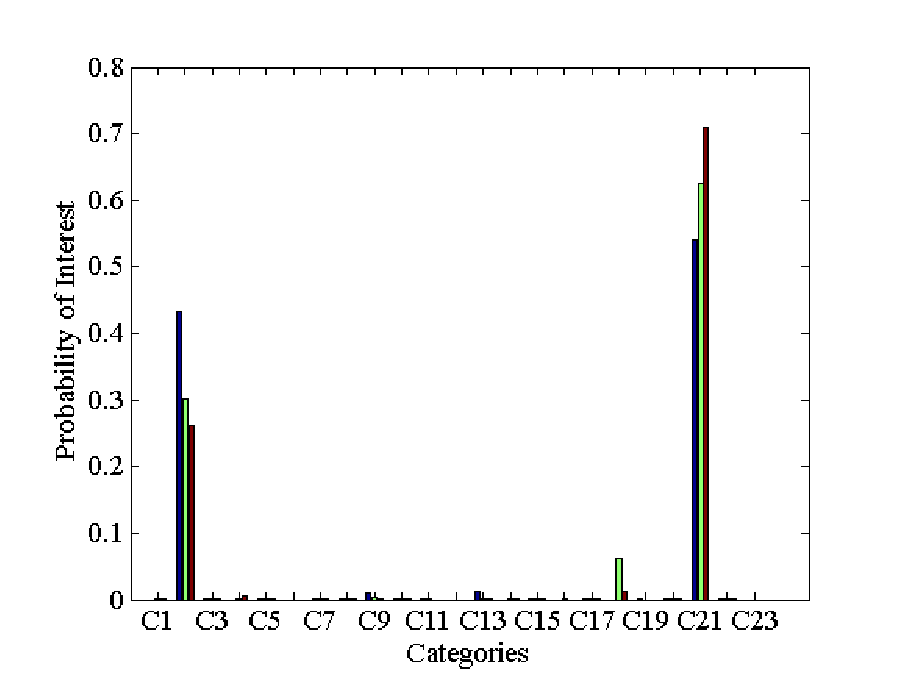
\includegraphics[width=8cm,height=3cm]{User2}} \caption{Sample profile PMFs for three users from LiveLab smart phone traces.\label{fig:SampleProfile} }
\end{figure}
 This finding invalidate the use of some metrics, such as Canberra
Distance and Jensen Shannon Divergence, with similar profiles. 
\par\end{flushleft}

We examine the Cosine, Hellinger, SVD and VCOS similarity metrics%
\footnote{Correlation is excluded because it has a different output range and
performing any mapping may skew the results. %
} to evaluate the pair-wise similarity for the $34$ LiveLab users,
which yields $561$ experiments. The outcomes of the four metrics
are shown, for the $561$ experiments, in the scatter plot depicted
in Fig.~\ref{fig:scatter}.
\begin{figure}[!bp]
%    \centering


\raggedright{}\centerline{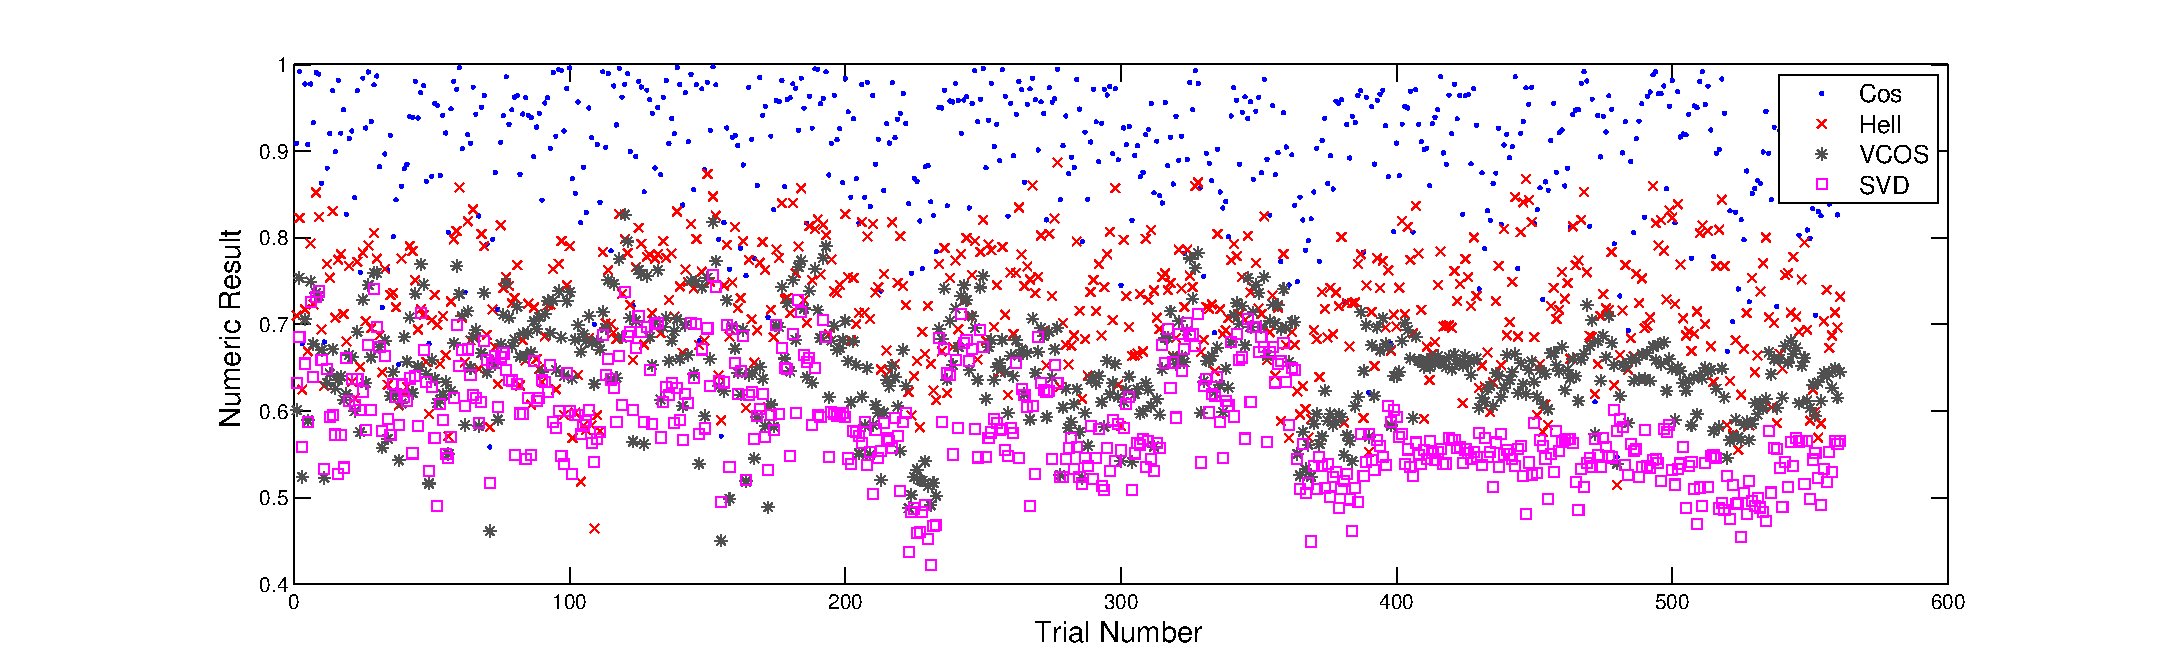
\includegraphics[width=9.5cm,height=4cm]{all}}
\vspace{-0.5cm}
 \caption{Metric indices for pair-wise similarity between LiveLab users.\label{fig:scatter}}
\end{figure}
 Few observations are now in order. It can be noticed that the Cosine
and Hellinger similarity yield relatively higher metric values compared
to the VCOS and SVD for the same pair of users. This interesting result
confirms the intuition that temporal metrics are generally \textquotedbl{}more
conservative\textquotedbl{} in assessing mobile user similarity. Thus,
for a given threshold $T$, two users may be perceived ``similar\textquotedbl{}
using a non-temporal metric, yet, ``dissimilar\textquotedbl{} using
a temporal metric. This is attributed to the fact that the temporal
profiles bear, naturally, more details and dynamics than the non-temporal
ones. This result is quantitatively shown in Table \ref{tab:Percentage-of-similar}.
\begin{table}
\tabcolsep=0.05cm \caption{Percentage of similar users for all metrics while varying the similarity
threshold.\label{tab:Percentage-of-similar}}


\centering{}{} \label{tab:NonAndTemporal-Maj} %
\begin{tabular}{|l|l|l|l|l|l|l|l|l|l|l|}
\hline 
 & 0.1 & 0.2  & 0.3  & 0.4  & 0.5  & 0.6  & 0.7  & 0.8  & 0.9  & 1\tabularnewline
\hline 
SVD  & 100  & 100  & 100  & 100  & 92.51  & 34.41  & 3.57  & 0  & 0  & 0\tabularnewline
\hline 
VCOS & 100  & 100  & 100  & 100  & 98.93  & 80.93  & 18.36  & 0.3565  & 0  & 0\tabularnewline
\hline 
Hell & 100  & 100  & 100  & 100  & 99.82  & 92.87  & 61.5  & 13.37  & 0  & 0\tabularnewline
\hline 
Cos & 100  & 100  & 100  & 100  & 100  & 99.47  & 97.33  & 89.13  & 59.18  & 0\tabularnewline
\hline 
\end{tabular}
\end{table}
 It shows that VCOS and SVD yield a lower percentage of similar users
than the Cosine and Hellinger metrics, hence, they are more conservative. 

Based on the observations discussed earlier, we envision two similarity
assessment paradigms, namely macroscopic (non-temporal based) and
microscopic (temporal-based). \textit{Macroscopic assessment:} quantifies
similarity between two vector-based, non-temporal profiles. Evidently,
it is less complex and faster, yet, somewhat looser. Hence, it is
compelling as a ``coarse-grained\textquotedbl{} similarity filter.
This paradigm resembles getting to know a person quickly, yet, superficially.
\textit{Microscopic assessment:} quantifies similarity between two
matrix-based, temporal profiles. Unlike the first paradigm, it is
more conservative in establishing similarity at the expense of more
complexity and, hence, being slower. This paradigm resembles knowing
a person deeply and more thoroughly.

\begin{comment}
 Section II is dedicated to our novel profile structures based on
probability distribution. Afterwards, we study the problem of similarity
between probability distribution, temporal and non-temporal, mobile
user profiles and introduce the novel vectorized similarity metric
for temporal profiles in Section III. Our performance analysis, major
findings and discussion are presented in Section IV. Finally, we draw
conclusions and point out potential directions for future research
in Section V
\end{comment}


\begin{comment}
The tight coupling between devices, users and networks has been leveraged
in \citet{profilecast,csi} to deliver messages to a group of users
specified by their behavioral profile (percentage of time spent within
each access point (AP) coverage). However, this captures only mobility
behavior exploited to improve the overall network performance. In
\citet{csi}, an extensive analysis of campus WiFi traces has shown
that users tend to cluster heavily in groups based on long-term similarity
of network access behavior. Moreover, each group tends to frequent
very few locations.\\
\\
\%The form of communication that is based on similarities and common
interests have been previously adopted in dating applications as in
\textbackslash{}cite\{lbd\} where a user can lookup who else is in
proximity and depending on common interests can decide to communicate
\textbackslash{}cite\{ms\}. Attempts to measure the similarity between
users in social contexts, which are based on spatio-temporal proximity
(i.e. being in the same place at the same time), are proposed in \textbackslash{}cite\{stp\},
in the context of tourism applications. However, the focus of \textbackslash{}cite\{stp\}
is limited to collaborative filtering and the concept of spatio-temporal
similarity. Our similarity notion extends to include temporal-based
profile structure and similarities. The previously mentioned applications
(dating and tourism) are examples of proximity based services. Trust
establishment between users depending on similarity are studied in
the context of online communities \textbackslash{}cite\{corr\} and
in the context of mobile societies \textbackslash{}cite\{protect\}.
\end{comment}
{} 

\begin{comment}
Our contribution in this paper is multi-fold. First, we extend mobile
user profiles, beyond mere location, to a generalized probability
distribution function, with non-temporal and temporal versions. Second,
we distill key insights about known and proposed temporal and non-temporal
similarity metrics, using publicly available data sets \citet{data}.
Third, we identify the Hellinger distance as a strong candidate for
quantifying similarity due to the probability distribution structure
of the proposed profile. Finally, we propose a novel temporal similarity
metric, based on matrix vectorization, to capitalize on the richness
in the temporal dimension and circumvent the limitations of prior
temporal similarity metrics \citet{csi}.
\end{comment}


\bibliographystyle{IEEEtran}
\bibliography{KG_References}

\end{document}
